\chapter{Crystal Processing}
The manufacturing process of a planar HPGe detector begins with a slice from a crystal boule that has been tested for quality and is know to be detector grade.
Typical boules slices are solid discs that can range from a few millimeters up to several centimeters in thickness and more than 5 centimeters in diameter.
This large size allows for several detector samples to be cut from each slice so careful geometry considerations are important in order to minimize wasted material.
The goal is for the detector sample to look approximately like figure \ref{fig:dummydet} which is an example of a planar detector with so called top hat geometry.
\begin{figure}[htpb]
\centering
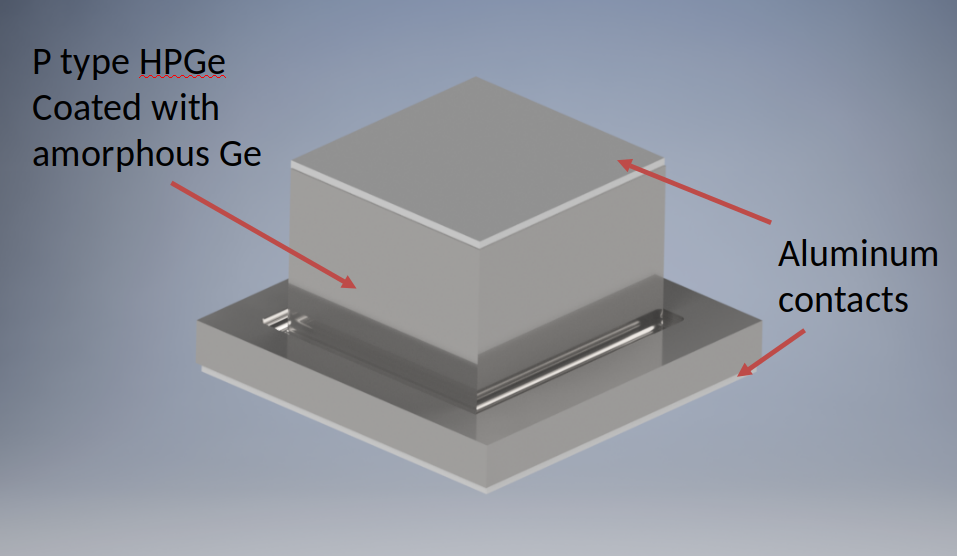
\includegraphics[width=0.5\textwidth]{dummy-det}
\caption{Example detector geometry with four wings}
\label{fig:dummydet}
\end{figure}
The brims of the hat are called wings and serve as a dead area of the detector for handling during the manufacturing process.
The detector is not required to be perfectly square to work so length and width can vary within a few centimeters.
What is of importance are the overall thickness and that the top and bottom faces are parallel.
Due to the relatively long mean free path of gamma rays in germanium, a detector should aim to be at least one centimeter thick.

Once considerations for geometry have been made, the detector manufacturing process begins.
To start, the germanium boule slice is cut into several rectangular cubes using a diamond CNC saw.
Then, work proceeds using one of the cubes, saving the others for next time.
The cube is further cut and ground to the top hat shape shown in Fig.~\ref{fig:dummydet}.
After cutting, the sample is lapped, polished, and then undergoes a chemical etching after which it is ready for thin film deposition.

Sometimes detectors will end up breaking down or failing completely.
Thus it is necessary to understand the properties of the germanium at every step of the manufacturing process.
A key method to quality insurance is to understand surface properties and how they change during mechanical and chemical processing as well as the thin film thicknesses.
To measure and analyze these, an optical microscope and a surface profiler are used.

\section{Mechanical Processing}
The diamond saw under discussion is the SYJ-400 Precision CNC Dicing/Cutting Saw from Shenyang Kejing Auto-Instrument Co.
The structure of this diamond saw is shown in Figure \ref{fig:diamondsaw}.
It is operated using a CNC controller with setting for the cutting speed, length, time, depth, lifting height, rest time, and movement speed.
All of these parameters are edited using the attached CNC controller. 
There are four separate screens with adjustable parameters that are shown with translations in Figure \ref{fig:control-screen}. 
Each of these parameters are in millimeters or millimeters per minute depending on the operation.
\begin{figure}[htpb]
\centering
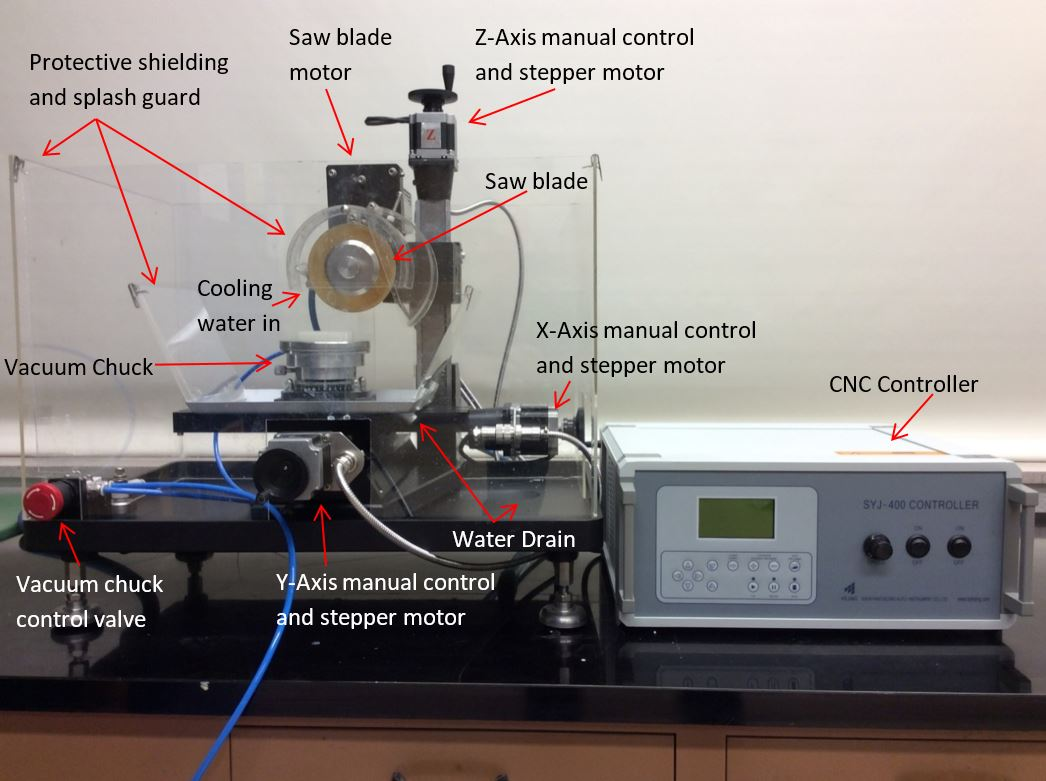
\includegraphics[width=0.8\textwidth]{diamond-saw}
\caption{The diamond saw used to cut boules into detector samples.}
\label{fig:diamondsaw}
\end{figure}

There are currently three different blades available for cutting.
They are all four inches in diameter and include: an electroplated diamond blade, full sintered diamond blade, and a 2mm grinding wheel.
The electroplated blade is thin and useful for the initial cuts of the boule.
The grinding wheel is used to make grooves and grind down the detector wings.

The next step is to mount the sample onto the vacuum chuck.
It is essential to do this before powering on the diamond saw to avoid accidents.
The sample is glued on top of a block of graphite using melt sticky wax. The graphite block is glued on top of a steel sample holder using the melt wax as well.
The steel sample holder is then placed onto the vacuum chuck and adjusted so it is properly aligned.
A vacuum pump is turned on to suck the sample holder, which keeps the sample from moving during cutting.
The next step is to power on the up/down converter, which provides a stepped up voltage (from 110~V to 220~V) to the CNC controller (which powers the saw).
The saw controller requires 220 volts which is why it cannot be plugged into a standard outlet.

The first cuts of the boule should be made with the thin diamond blade and go all the way through the germanium into the graphite plate.
The initial cuts are to cut the rough detector shape out of the crystal slice.
An example of a cut boule can be seen in Figure ~\ref{fig:cutboule} where four detector samples are cut from a single slice of a crystal boule.
\begin{figure}[htpb]
\centering
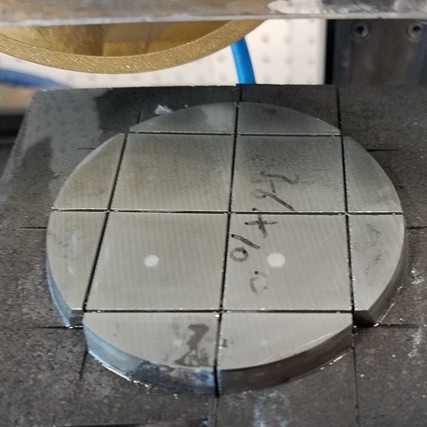
\includegraphics[width=0.5\textwidth]{cut-boule}
\caption{A slice of crystal after the initial detector sample blanks have been cut.}
\label{fig:cutboule}
\end{figure}
The saw must be started and stopped using the provided controller.
All of the settings and translations can be seen in the appendix in Figure ~\ref{fig:control-screen}.
One property of germanium is that it is extremely brittle.
This can cause problems during cutting because the material will chip if it is cut too fast.
Due to this problem, the diamond saw must travel less that a millimeter per minute and grind the germanium instead of cutting it.

After the detector blanks have been cut from the boule, the steel sample holder and graphite plate are reheated to melt the wax and remove all the extra pieces.
A single detector sample is then left and centered on the graphite for further cutting.
The next step is to replace the thin blade with the grinding wheel so that the groove cuts can be made.
A detector can have either two or four wings depending on the final goal.
The groove are ground out approximately two millimeters from the edge of the sample, then the sample is moved and the remaining bits are ground down to leave the wing shape.
An example of a detector with four wings is shown in Figure ~\ref{fig:cut-sample}.
\begin{figure}[htpb]
\centering
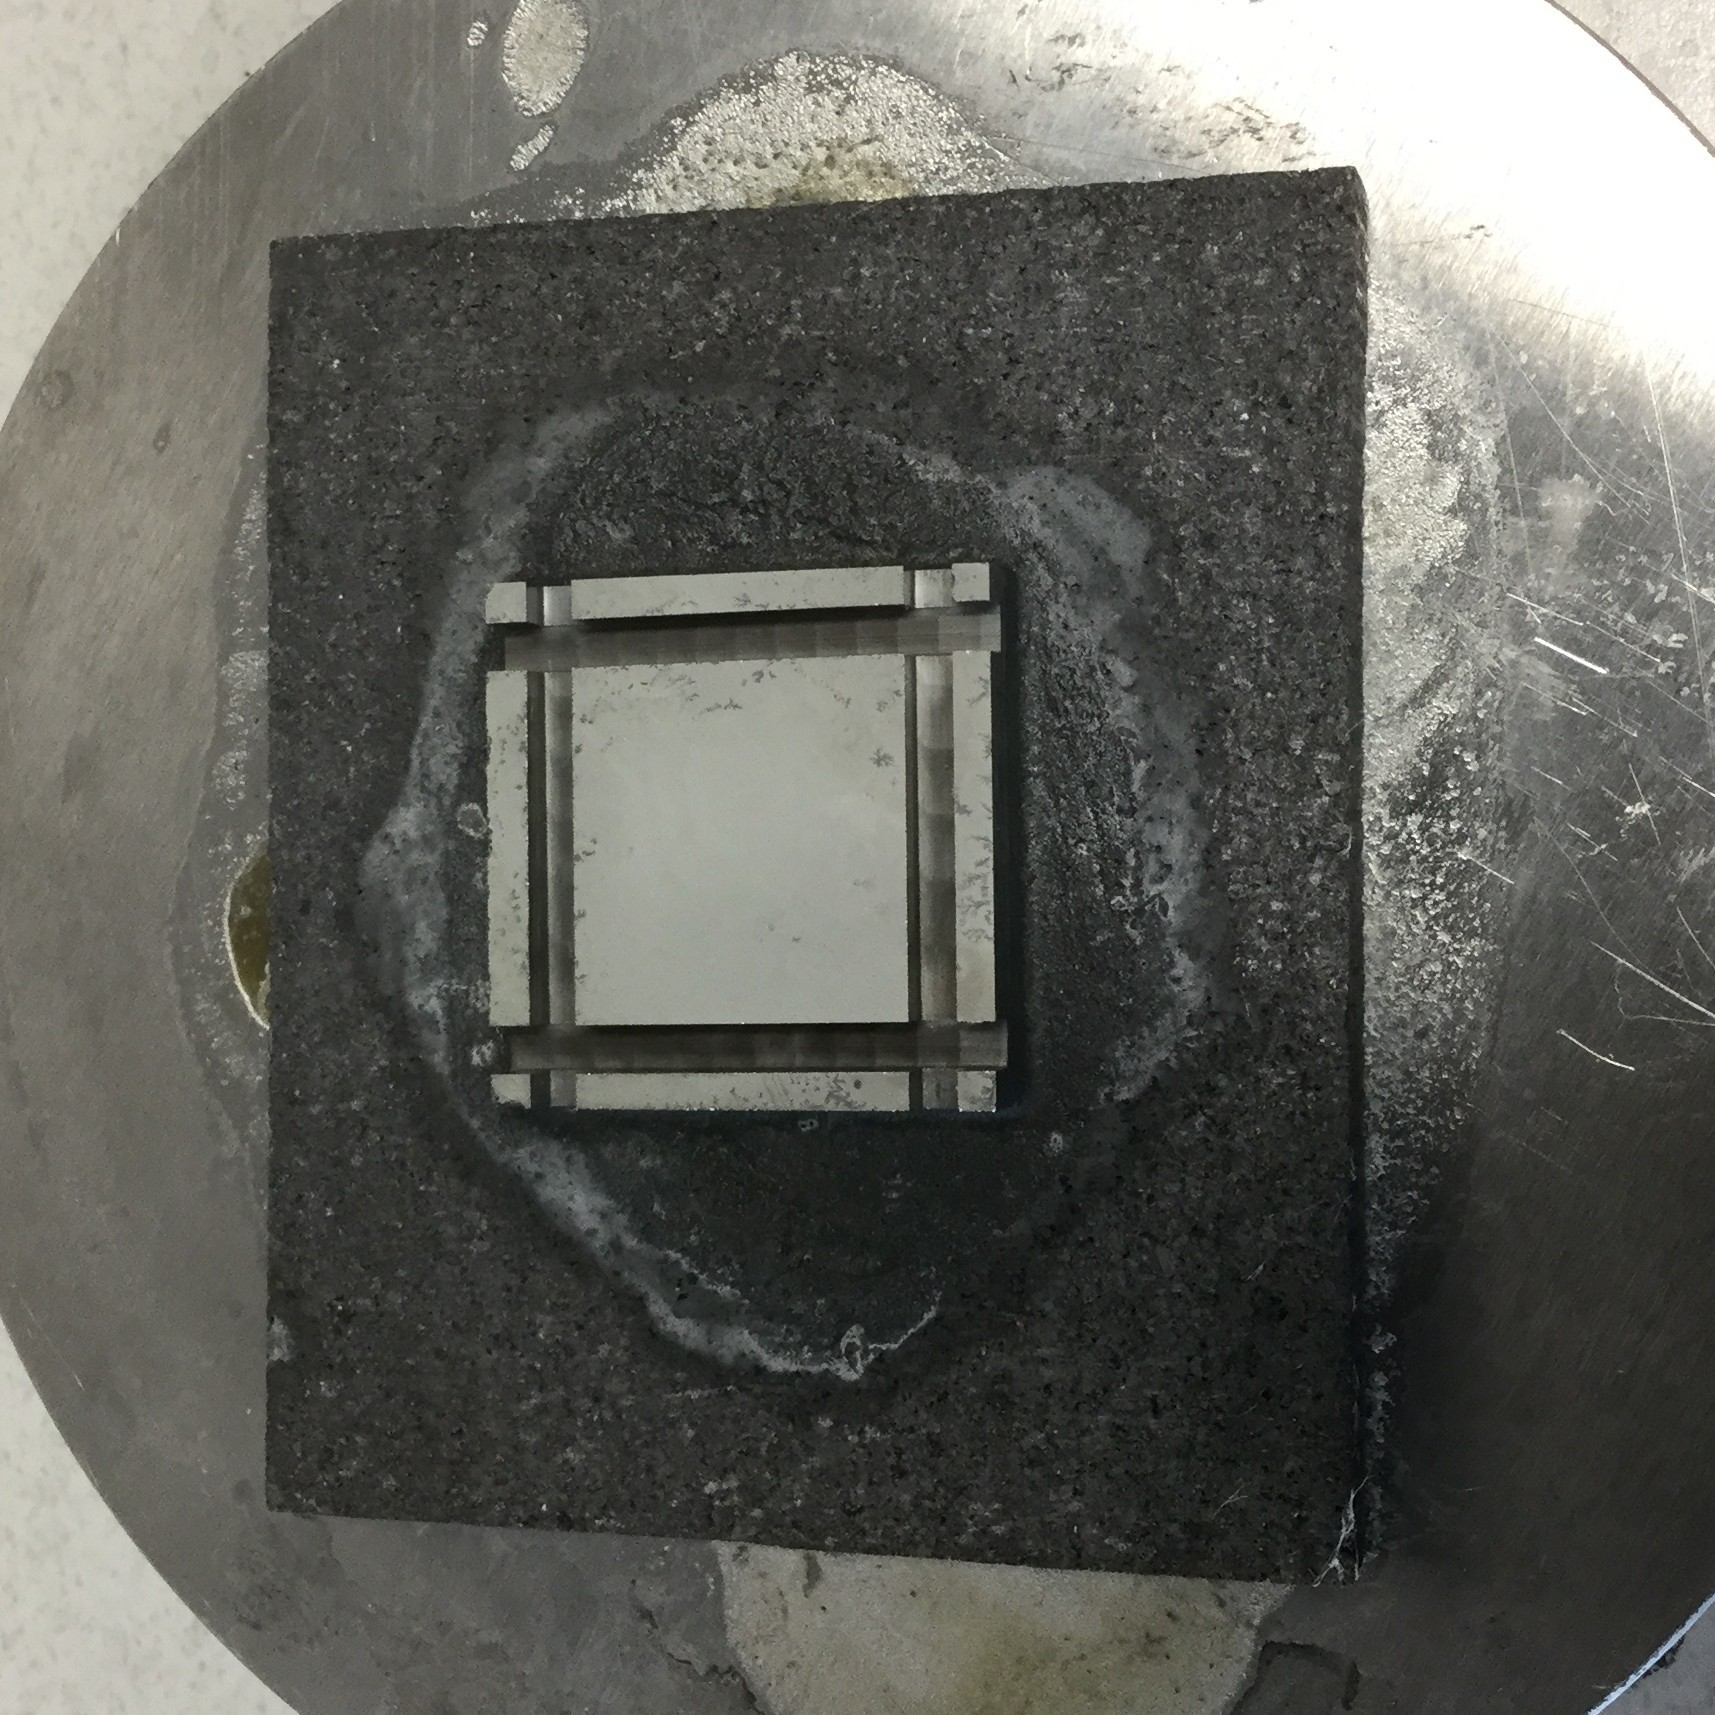
\includegraphics[width=0.5\textwidth]{cut-sample}
  \caption{A germanium sample mounted on graphite which is then mounted on a stainless steel chuck (sample holder).}
\label{fig:cut-sample}
\end{figure}

After the detector has finished up in the diamond saw, it is left with a very rough surface that might have some minor chipping along the edge.
Any cracks or large chips can lead to detector failure down the line so they must be removed before continuing.
The first and most effective way to remove material is through lapping.
For lapping, an abrasive is mixed with water on a glass plate to create a slurry.
The standard procedure is to spoon out a few grams of the abrasive onto the glass slide.
Then enough DI water to create a slurry is mixed into the powder.
The detector is then ran across the slurry which slowly grinds down the surface.
The speed of material removal is based on the type and particle size of the abrasive.
Two types of abrasives are used for lapping at USD, one is silicon carbide (SiC) and the other is aluminum oxide (Al$_2$O$_3$).
To remove lots of material, the larger grit SiC is used.
The brand ID is Lapmaster 2600 and it has an average particle size of 17.5 micron.
For finer lapping the aluminum oxide with average particle size of 9.5 micron is used.
The Al$_2$O$_3$ is available in several particle sizes where the most used at USD are the 9.5 micron (Lapmaster 1900) and 1 micron versions.
Generally the 9.5 micron Al$_2$O$_3$ is enough to remove major defects from the diamond saw.
Occasionally further polishing is required to reduce the amount of time required for chemical processing.
In order to achieve a mirror like finish prior to acid etching, a polishing pad can be used.
When using the polishing pad, shown in Figure \ref{fig:lapping}, it is important to use an abrasive of 3 microns or less to achieve a nice finish.
Figure \ref{fig:lapping} shows a polishing pad with a detector sitting in the slurry.
\begin{figure}[htpb]
\centering
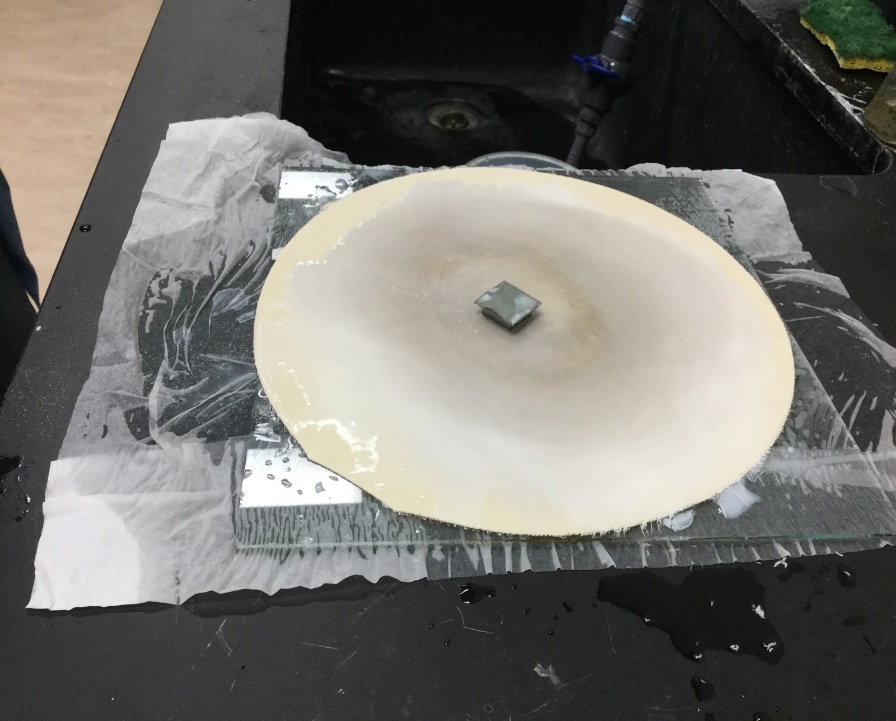
\includegraphics[width=0.5\textwidth]{lapping}
\caption{Polishing a detector sample.}
\label{fig:lapping}
\end{figure}

\section{Chemical Processing}

The cutting and lapping leaves the surface of the detector with micro scratches and defects, sometimes invisible to the naked eye, that could lead to failure down the process line if not treated properly.
Since the next step of detector fabrication involves depositing thin layers of metal that need to stick together, it is important that the surface is as smooth and clean as possible.
Acid etching is a useful tool to remove the outer layer of germanium and leave behind a smooth and defect free surface as long as the right chemical mixture is used.  

Several chemical treatments are commonly used in the semiconductor industry to deal with such cleaning and polishing.
For cleaning there are solvents such as acetone, methanol, and Trichloroethylene that are used to remove the wax and debris after cutting.
The detector manufacturing lab is equipped with a metal hood for such operations involving these solvents that is shown in Figure ~\ref{fig:metalhood}
\begin{figure}[htpb]
\centering
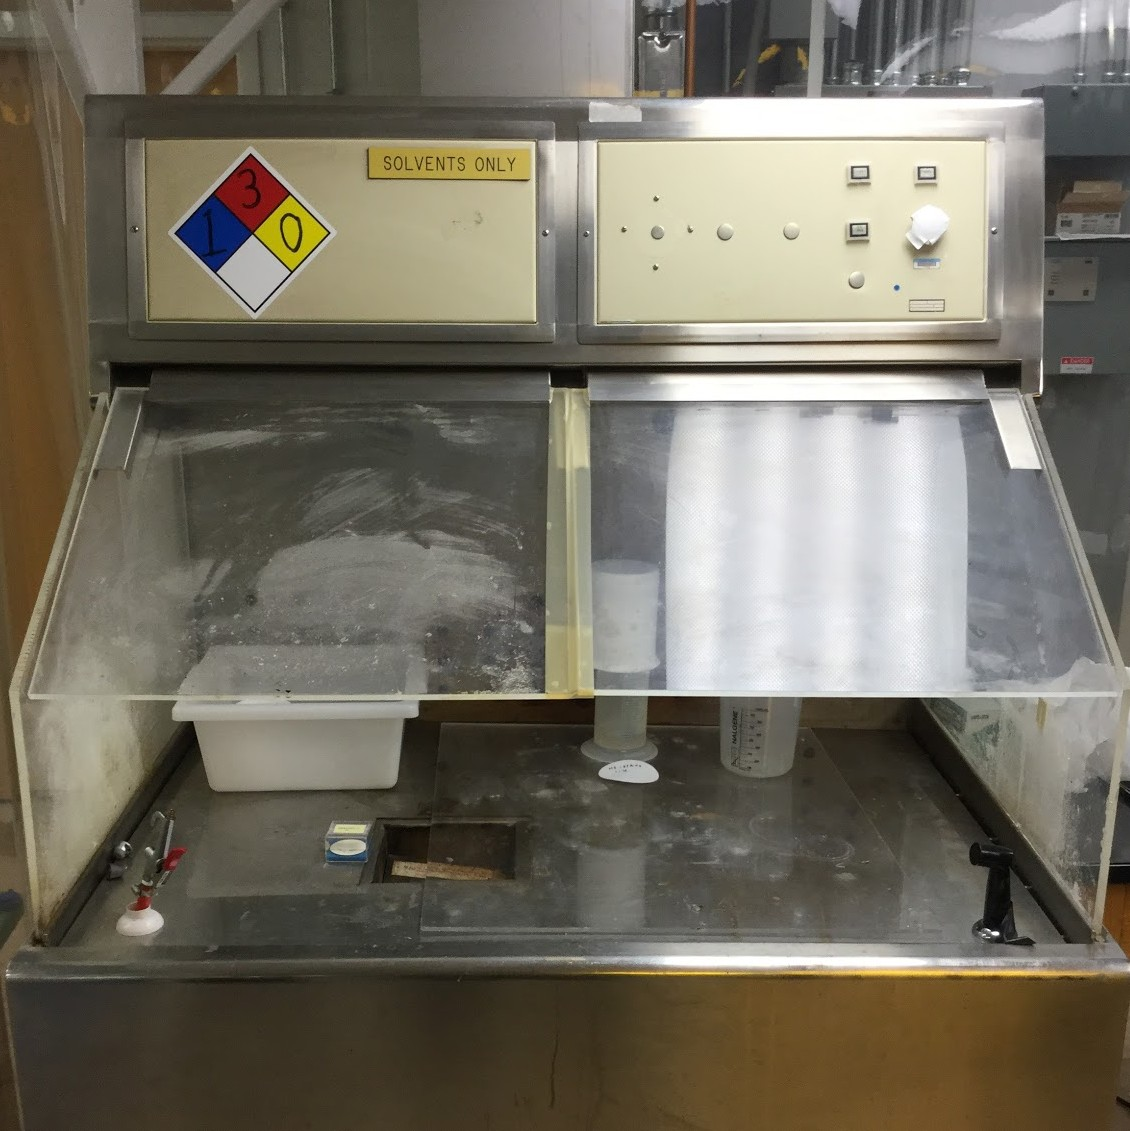
\includegraphics[width=0.5\textwidth]{metal-hood}
\caption{Metal hood for use with solvents.}
\label{fig:metalhood}
\end{figure}

Usually a mixture of Nitric (HNO$_3$) and hydrofluoric (HF) acids is used for etching.
The ratio of the two acids will determine how aggressive the etching is.
For detector fabrication a 4:1 HNO$_3$(100\%):HF(49\%) ratio is used.
Figure \ref{fig:plastichood} shows the plastic hood that is used for acid etching.
\begin{figure}[htpb]
\centering
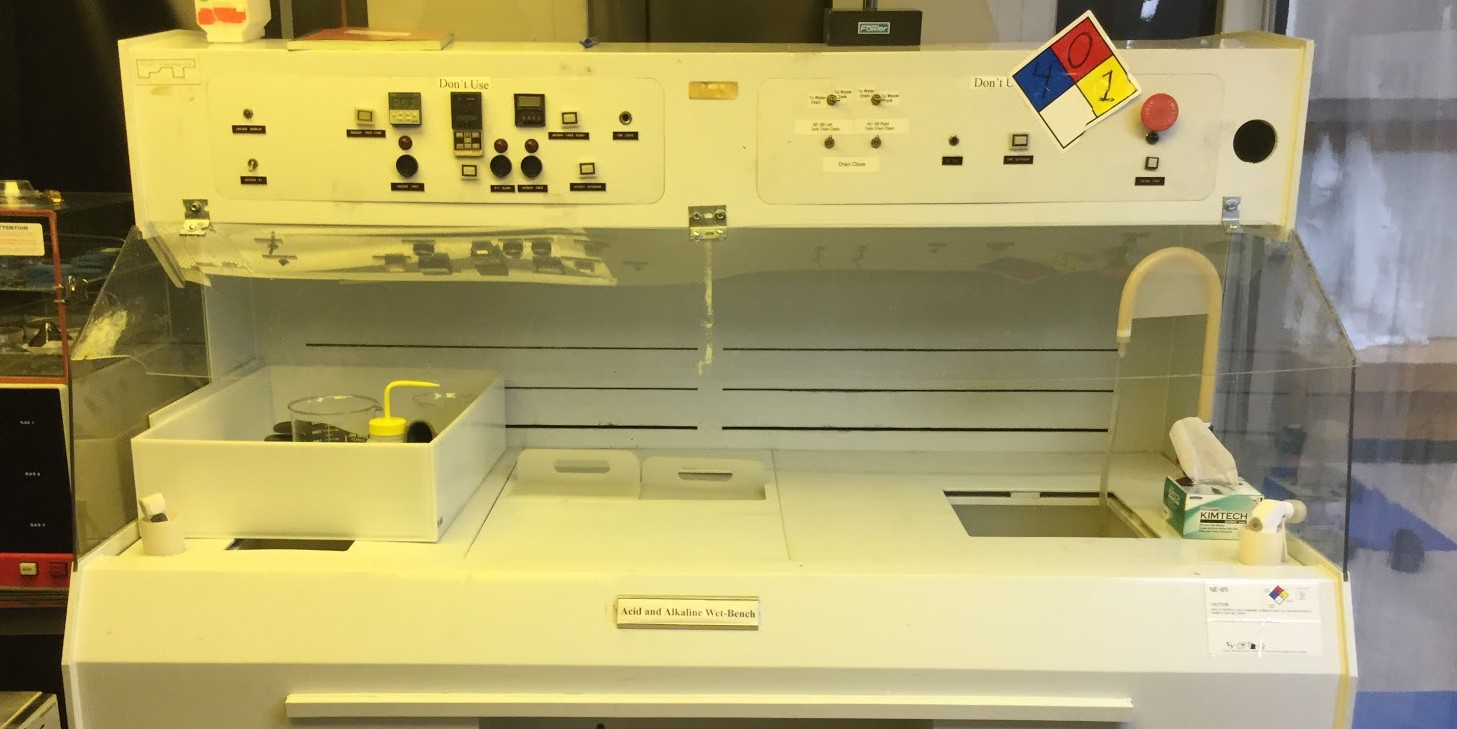
\includegraphics[width=0.7\textwidth]{plastic-hood}
\caption{Plastic hood for use with acids.}
\label{fig:plastichood}
\end{figure}
To prepare for sputtering and aluminum deposition, two etches are required.
Both etches are in the 4:1 solution, however, the time varies.
The first etch is around three minutes long and takes place after lapping.
This longer etch is meant to fully polish the crystal and rid it of scratches and defects.
The second etch is only 30 seconds and is to clean the surface of the crystal immediately before it is loaded into the sputtering machine.

The procedure for acid etching starts with taking proper precautions to ensure safety and prevent accidents.
HF-resistant gloves are worn on top of of lab gloves, along with safety goggles, lab coat, and respirator if necessary.
Then the acid mixture can be made.
Figure \ref{fig:acidbeakers} shows the acid bottles along with several beakers and a graduated cylinder.
The graduated cylinder is used to measure out the proper ratio of acids, usually 160 ml of nitric acid is poured in first followed by 40 ml of hydrofluoric.
This is enough solution for at least two etches.
Approximately 100 ml of solution is then poured into an empty PTFE beaker.
It is also necessary to have at least three beakers filled with DI water, two for quenching after the etch and one two quench any paper waste.
\begin{figure}[htpb]
\centering
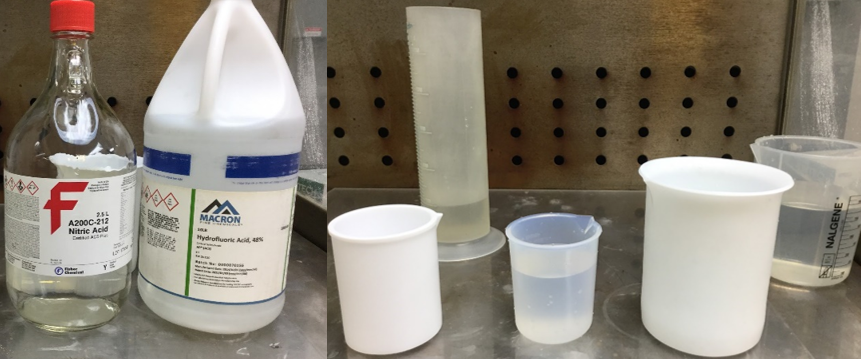
\includegraphics[width=\textwidth]{acidbeakers}
\caption{Left: Nitric and Hydrofluoric acid bottles. Right: Graduated cylinder PTFE and plastic beakers.}
\label{fig:acidbeakers}
\end{figure}
After the setup is complete, etching can proceed.
For the longer three minute polish, the clean detector sample is placed in the acid using long acid resistant tweezers.
The detector must then be continuously agitated and flipped halfway through to ensure a uniform etch.
After the three minutes have elapsed the detector is removed and immediately dipped into the first DI water beaker for a few seconds to stop the etch.
Then it is dipped into the second DI water beaker to remove any remaining acid.
After the DI water quench, the detector is quickly dried with nitrogen gas to remove all moisture from the surface.
The surface of the detector sample should now have a mirror finish, although some minor cloudiness sometimes arises and is acceptable.
If scratches remain, the detector can be etched further, usually for a minute or less.
\begin{figure}[htpb]
\centering
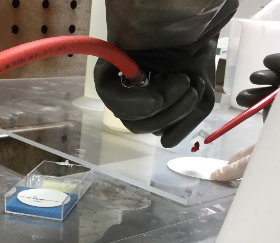
\includegraphics[width=0.5\textwidth]{drynitrogen}
\caption{A detector sample being held and dried with nitrogen.}
\label{fig:drynitrogen}
\end{figure}

At this point the detector sample is ready for the final 30 second etch and loading into the sputtering machine.
The same etch mixture is used as in the long etch, only this time the sample is held continuously by the tweezers and is swished around in the acid.
Being held continuously prevents the surface from contacting anything other than acid and keeps it free from the possibility that more scratches are introduced.
The steps of quenching in DI water and drying with nitrogen are the same with importance being placed on the sample being held and never allowed to touch any surfaces.
After the detector sample is dried, it can be placed onto the sputtering jig and loaded into the sputtering machine.


